\documentclass[12pt, a4paper]{report}

% Импорты 

\usepackage{cmap}
\usepackage{url}
\usepackage{hyperref}
\usepackage{amsthm, amsmath, amssymb}
\usepackage{thmtools}
\usepackage{fancyhdr}
\usepackage{graphicx}
\usepackage{titlesec}
\usepackage[normalem]{ulem}
\usepackage{cancel}
\usepackage{subcaption}

\usepackage[english, russian]{babel}
\usepackage[utf8]{inputenc}
\usepackage[T2A]{fontenc}

% Геометрия 

\usepackage{geometry}
\geometry{
	left=1.5cm,
	right=1.5cm,
	top=2cm,
	bottom=1.5cm
}

\setlength\parindent{0pt}

% Теоремы, леммы ...

\renewcommand{\listtheoremname}{Список теорем}

\newtheorem{theorem}{Теорема}[section]
\newtheorem{lemma}[theorem]{Лемма}
\newtheorem{corollary}[theorem]{Следствие}
\theoremstyle{definition}
\newtheorem*{definition}{Определение}
\theoremstyle{remark}
\newtheorem{remark}[theorem]{Замечание}
\newtheorem{example}[theorem]{Пример}
\theoremstyle{remind}
\newtheorem*{remind}{Remind}

\newcommand{\divisible}{\mathop{\raisebox{-2pt}{\smash{\vdots}}}}
\newcommand{\notdivisible}{\mathop{\raisebox{-2pt}{$\not \vdots$ }}}

% Колонтитулы

\pagestyle{fancy}
\fancyhf{}
\fancyhead[R]{\rightmark}
\fancyhead[L]{\textsc{\thechapter. \leftmark}}
\fancyfoot[C]{\thepage}
\renewcommand{\chaptermark}[1]{\markboth{#1}{}}
\renewcommand{\sectionmark}[1]{\markright{#1}}

% Главы

\titleformat{\chapter}[display]
{\normalfont\huge\bfseries\centering} % Формат текста
{\titlerule[1pt] \vspace{1pt} \titlerule\vspace{1pc} \Huge\MakeUppercase{\chaptertitlename} \thechapter} % Номер главы
{1pc} % Отступ между номером главы и названием
{\Huge} % Формат названия главы
[\vspace{1pc} \titlerule] % Декоративные элементы после названия

\titlespacing*{\chapter}{0pt}{0pt}{40pt}

\begin{document}
	
	\begin{titlepage}
		\newgeometry{left=1.5cm, right=1.5cm, top=3cm, bottom=2cm}
		\centering
		
		{\Large Санкт-Петербургский губернаторский\\ Физико-математический лицей №30}\\[1cm]
		
\includegraphics[width=0.18\textwidth]{assets/logo.png}\\[5cm]
		
		\textbf{ \LARGE Конспект уроков алгебры 9-го класса}\\[2cm]
		
		\begin{flushright}
			\textbf{Ученика:} \\ Лавелина М.Е. \\[1cm]
			\textbf{По мотивам уроков:} \\ Ренёва О.В. \\[1cm]
		\end{flushright}
		
		\vfill
		
		{\large 2024--2025 г.}
		
	\end{titlepage}
	
	\begin{abstract}
		Я пишу для себя так, понятно и удобно мне. Некоторые формулировки могут быть не точными или вовсе не верными. 
		Думайте прежде всего \textbf{своей} головой. \\

		
		\begin{center}
		  Удачи в изучении алгебры!
		\end{center} 
		
	  \end{abstract}

	\newgeometry{left=1.5cm, right=1.5cm, top=1cm, bottom=2cm}
\tableofcontents
\setcounter{page}{0} 
\thispagestyle{empty}
\restoregeometry
	
	\chapter{Пример главы}

\section{Степень с целым показателем}

\begin{definition}
    \[
        m \in \mathbb{Z}: \; a^m = 
        \left\{
        \begin{array}{l}
            a^m, \; m \in \mathbb{N} \\ \\
            1, \; m = 0 \\ \\
            \frac{1}{a^m}, \; m \in  \mathbb{Z} \land n < 0 \\
        \end{array}\right.
    \]
\end{definition}

\begin{remark}
    $a^m$, при $m \in \mathbb{Z} \; \backslash \; \mathbb{N}$ не определенно при $a = 0$. Иными словами, ноль нельзя возводить в неположительную степень.
\end{remark}

\begin{example}
    $2^{-3} = \frac{1}{2^3} = \frac{1}{8}$; $(\frac{3}{2})^{-2} = \frac{2^2}{3^2} = \frac{4}{9}$;
\end{example}

\begin{theorem}
    $\forall a \in \mathbb{R} \backslash \{0\} \; \forall m, n \in \mathbb{Z}: \; a^m \cdot a^n = a^{m + n}$
\end{theorem}

\begin{proof}
    \hfill

    \begin{enumerate}
        \item $m,n \in \mathbb{N}$ - см. доказательство для $\mathbb{N}$
        \item $m = 0 \lor n = 0$ - очевидно
        \item $m < 0 \land n > 0$:
        \begin{align*}
            a^m \cdot a^n = \frac{a^n}{a^{-m}} = a^{n - (-m)} = a^{m + n}
        \end{align*}
        \item $m > 0 \land n < 0$:
        \begin{align*}
            a^m \cdot a^n = \frac{a^m}{a^{-n}} = a^{m - (-n)} = a^{m + n}
        \end{align*}
        \item $m < 0 \land n < 0$:
        \begin{align*}
            a^m \cdot a^n = \frac{1}{a^{-n} \cdot a^{-m}} = \frac{1}{a^{-(n+m)}} = a^{m + n}
        \end{align*}
    \end{enumerate}
\end{proof}

\break

\begin{theorem}
    $\forall a \in \mathbb{R} \backslash \{0\} \; \forall m, n \in \mathbb{Z}: \; (a^m)^n = a^{m \cdot n}$
\end{theorem}

\begin{proof}
    \hfill

    \begin{enumerate}
        \item $m,n \in \mathbb{N}$ - см. доказательство для $\mathbb{N}$
        \item $m = 0 \lor n = 0$ - очевидно
        \item $m < 0 \land n > 0$:
        \begin{align*}
            (a^m)^n = \left(\frac{1}{a^{-m}}\right)^n = \frac{1}{a^{-m \cdot n}} = a^{m \cdot n}
        \end{align*}
        \item $m > 0 \land n < 0$:
        \begin{align*}
            (a^m)^n = \frac{1}{(a^m)^{-n}} = \frac{1}{a^{-m \cdot n}} = a^{m \cdot n}
        \end{align*}
        \item $m < 0 \land n < 0$:
        \begin{align*}
            (a^m)^n = \frac{1}{(a^m)^{-n}} \stackrel{3.}{=} \frac{1}{a^{-m \cdot n}} = a^{m \cdot n}
        \end{align*}
    \end{enumerate}
\end{proof}

\begin{theorem}
    $\forall a \in \mathbb{R} \backslash \{0\} \; \forall m, n \in \mathbb{Z}: \; \frac{a^m}{a^n} = a^{m-n}$
\end{theorem}

\begin{proof}
    \hfill

    \begin{enumerate}
        \item $m,n \in \mathbb{N} \land m > n$ - см. доказательство для $\mathbb{N}$
        \item $m,n \in \mathbb{N} \land m = n$ - очевидно (нулевая степень)
        \item $m,n \in \mathbb{N} \land m < n$:
        \begin{align*}
            \frac{a^m}{a^n} = \frac{1}{(\frac{a^n}{a^m})} = \frac{1}{a^{n - m}} = a^{- (n - m)} = a^{m - n}
        \end{align*}
        \item $m = 0 \lor n = 0$ - очевидно
        \item $m < 0 \land n > 0$:
        \begin{align*}
            \frac{a^m}{a^n} = \frac{1}{a^{n} \cdot a^{-m}} = \frac{1}{a^{n - m}} = a^{- (n - m)} = a^{m - n}
        \end{align*}
        \item $m > 0 \land n < 0$:
        \begin{align*}
            \frac{a^m}{a^n} = \frac{m}{(\frac{1}{a^{-n}})} = a^{m} \cdot a^{-n}= a^{m - n}
        \end{align*}
        \item $m < 0 \land n < 0$:
        \begin{align*}
            \frac{a^m}{a^n} = \frac{a^{-n}}{a^{-m}} = a^{-n - (-m)} = a^{m - n}
        \end{align*}
    \end{enumerate}
\end{proof}

\break

\begin{theorem}
    $\forall a, b \in \mathbb{R} \backslash \{0\} \; \forall m \in \mathbb{Z}: \; (ab)^m = a^m \cdot a^n$
\end{theorem}

\begin{proof}
    \hfill

    \begin{enumerate}
        \item $m \in \mathbb{N}$ - см. доказательство для $\mathbb{N}$
        \item $m = 0$ - очевидно
        \item $m \in \mathbb{Z} \land m < 0$:
        \begin{align*}
            (ab)^m = \frac{1}{(ab)^{-m}} = \frac{1}{a^{-m} \cdot b^{-m}} = a^m \cdot a^n
        \end{align*}
    \end{enumerate}
\end{proof}


	\chapter{Графики и функции}

\section{Иррациональные уравнения}

\begin{align*}
    a = b &\iff f(a) = f(b) \\
    &\Rightarrow - \text{ верно всегда}\\
    &\Leftarrow - \text{ верно, если функция инъективна}
\end{align*}

\begin{definition}[Инъективность]
    Функция называется инъективной на множестве $A$ (инъекция на множестве $A$), если различным значениям аргумента из множества $A$, 
    функция сопостовляет различные значения функции.

    \begin{align*}
        &A \subset D(f) \\
        &\forall x_1, x_2 \in A \;\;\; x_1 \neq x_2 \Rightarrow f(x_1) \neq f(x_2)
    \end{align*}
\end{definition}

\begin{remark}
    На основании теоремы "док-во от обратного":
    \begin{align*}
        &(x_1 \neq x_2 \Rightarrow f(x_1) \neq f(x_2)) \iff (f(x_1) = f(x_2) \Rightarrow x_1 = x_2)
    \end{align*}
\end{remark}

\hfill \newline

\begin{remark}
    График инъективной функции пересекается произвольной горизонтальной прямой не больше одного раза.
\end{remark}

\begin{theorem}[Достаточное условие инъективности]
    Если функция строго монотонна на множестве $A$, то она инъективна на множестве $A$.
\end{theorem}

\begin{proof}
    \begin{align*}
        &\text{Функция строго монотонна, значит } \\
        &\left[\begin{array}{l}
            x < y \iff f(x) < f(y) \\
            x > y \iff f(x) > f(y) 
        \end{array}\right. \Rightarrow
        (x \neq y \iff f(x) \neq f(y))
    \end{align*}
\end{proof}

\begin{remark}
    Обратное неверно!
\end{remark}

\begin{remark}
    Степенная функция с нечетным натуральным показателем -- инъекция на всей вещестенной оси, так как всегда возрастает. 
\end{remark}

\begin{remark}
    Возведение обоих частей уравнения в нечетную натуральную степень всегда будет равносильным преобразованием.
\end{remark}

\begin{remark}
    Степенная функция с четным натуральным показателем не является инъекцией на всей вещестенной оси. 
\end{remark}

\begin{example}
    \begin{align*}
        \text{Если } f(x) = x^4; \; x_1 = 2; \; x_2 = -2, \text{ то } x_1 \neq x_2, \text{ но } f(x_1) = f(x_2) = 16
    \end{align*}
\end{example}

\begin{remark}
    Степенная функция с четным натуральным показателем является инъекцией отдельно на множестве $(-\infty; \; 0]$ и $[0; \; +\infty )$ 
\end{remark}

\begin{remark}
    При возведении обоих частей уравнения в четную натуральную степень могут появится лишние решения.
\end{remark}

\begin{example}
    \begin{align*}
        &\sqrt{x + 2} = x \iff x + 2 = x^2 \iff x^2 - x - 2 = 0 \iff \\
        &\left[\begin{array}{l}
            \uwave{x = -1} \leftarrow \text{лишний корень}\\
            x = 2
        \end{array}\right.
    \end{align*}
\end{example}

\begin{remark}
    Если можем гарантировать, что обе части уравнения имеют одинаковый знак, то возведение их в четную натуральную степень
    будет равносильным преобразованием.
\end{remark}

\begin{example}
    \begin{align*}
        &\sqrt{x + 2} = x \underset{x \ge 0}{\iff} x + 2 = x^2 \iff x^2 - x - 2 = 0 \iff \\
        &\left[\begin{array}{l}
            x = -1 \\
            x = 2
        \end{array}\right. \underset{x \ge 0}{\iff}
        x = 2
    \end{align*}
\end{example}

\begin{example}
    \begin{align*}
        &\sqrt{2x + 7} - \sqrt{x + 3} = 1 \iff \sqrt{2x + 7} = \sqrt{x + 3} + 1 \iff \\
        &2x + 7 = 1 + 2\sqrt{x + 3} + x + 3 \iff 2\sqrt{x + 3} = x + 3 \iff\\
        &4x + 12 = x^2 + 6x + 9 \iff x^2 - 2x - 3 = 0 \iff
        \left[\begin{array}{l}
            x = 1 \\
            x = -3
        \end{array}\right.
    \end{align*}
\end{example}
\section{Свойства и графики степенной функции}

\begin{definition}
    Степенная функция -- функция вида $f(x) = x^n$
\end{definition}

\subsection{Натуральная нечетная степень}

$f(x) = x^n, \; n \in \mathbb{N}  \land n \notdivisible 2$

\begin{itemize}
    \item $D(f) = \mathbb{R}$
    можем подставить любое число
    \item $E(f) = \mathbb{R}$
    согласно теореме \hyperref[thm:1.2.3]{о корректности определения}
    \item $f \uparrow \mathbb{R}$\\
    \begin{align*}
        &\forall x_1, x_2 : x_1 > x_2 \\
        &f(x_1) - f(x_2) = x_1^n - x_2^n = \underbrace{(x_1 - x_2)}_{> 0} \underbrace{(x_1^{n-1} + x_1^{n-2}x_2 + x_1^{n-3}x_2^2 \; \dots \; x_1x_2^{n-2} + x_2^{n-1})}_{> 0 \text{ см. ниже}} \\
    \end{align*}
    1. $x_1 > x_2 \ge 0$ - очевидно \\
    2. $x_1 > 0 > x_2$ - очевидно, $x_1^n - x_2^n > 0$ \\
    3. $0 \ge x_1 > x_2$ - см. четность степеней \\ \\
    Тогда
    \begin{align*}
        f(x_1) - f(x_2) > 0 \Rightarrow f(x_1) > f(x_2)
    \end{align*}
\end{itemize}

\begin{remark}
    С ростом $n$ график стремится к <<качерге>>, круто падая до $-1$ и круто растя после $1$
\end{remark}

\newpage

\begin{figure}[h]
    \centering
    \begin{subfigure}{0.35\textwidth}
        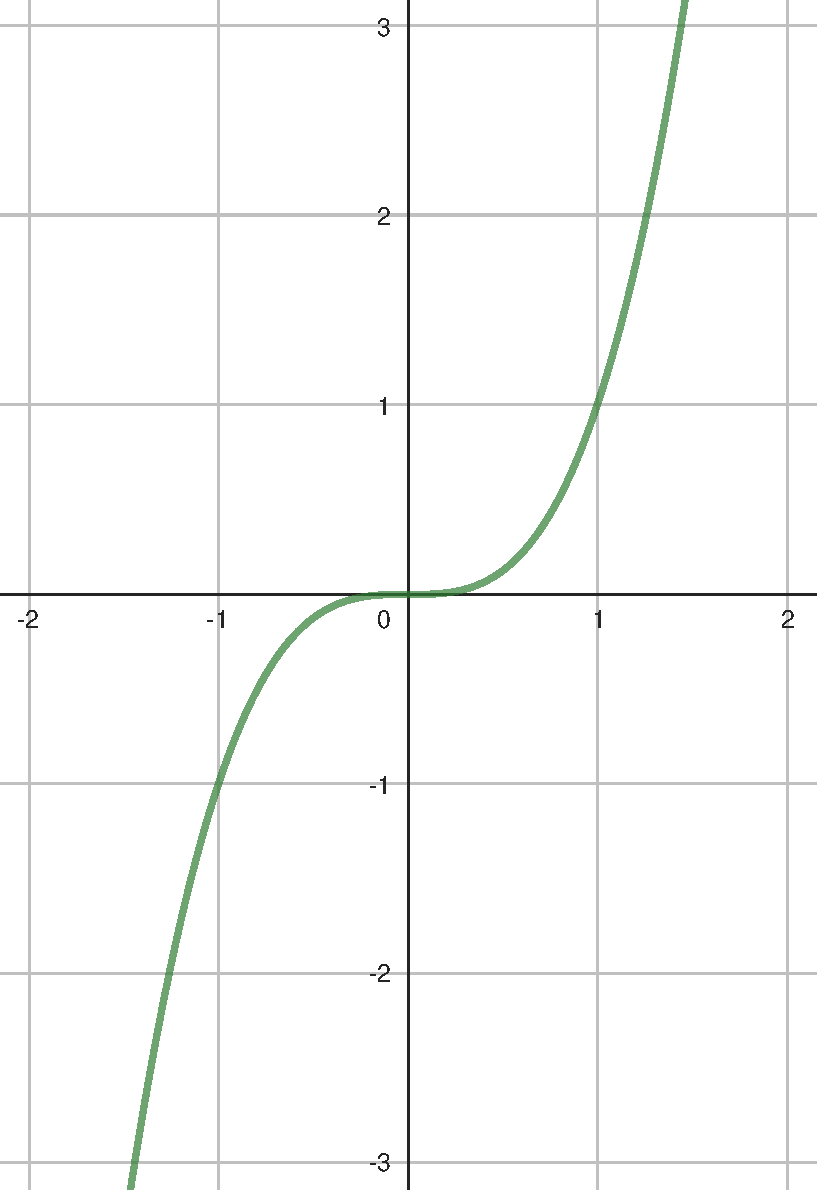
\includegraphics[width=\textwidth]{tex/chapter_2/assets/y=x^3.pdf}
        \caption*{$f(x) = x^3$}
    \end{subfigure}
    \hfill
    \begin{subfigure}{0.35\textwidth}
        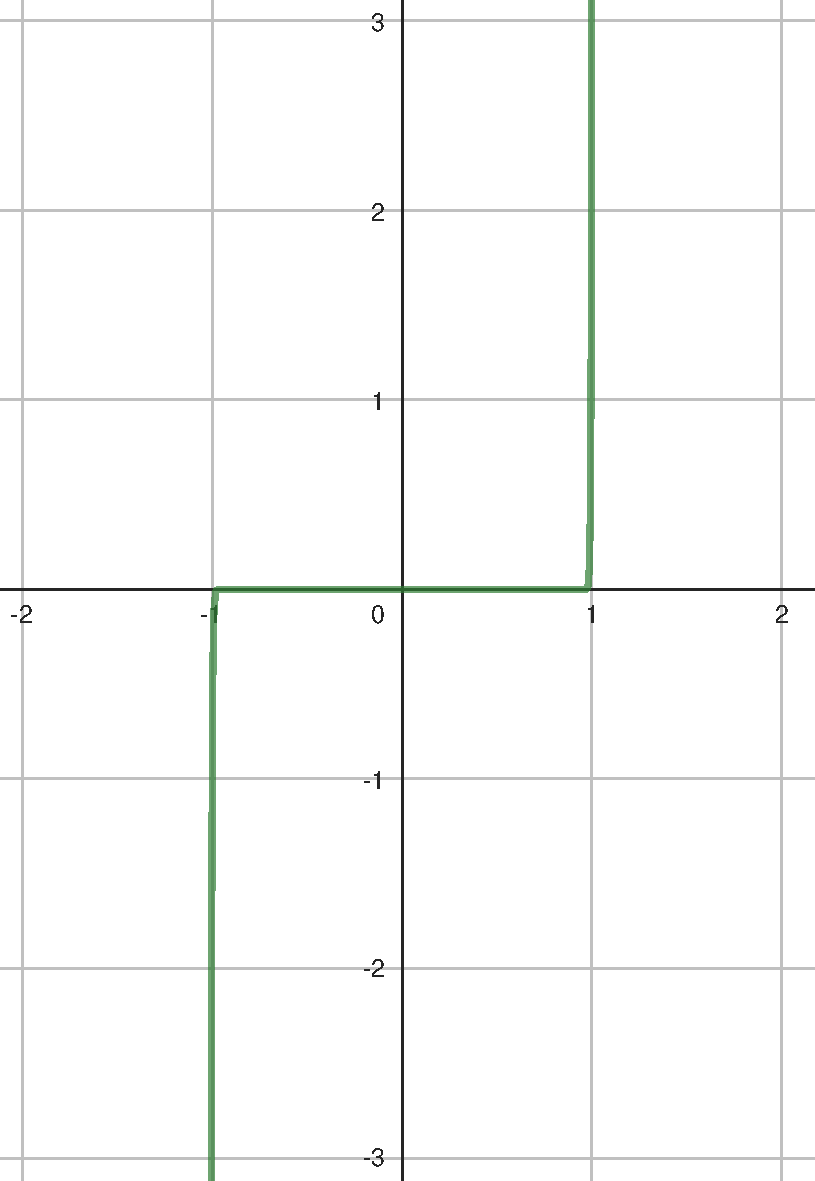
\includegraphics[width=\textwidth]{tex/chapter_2/assets/y=x^239.pdf}
        \caption*{$f(x) = x^{239}$}
    \end{subfigure}
\end{figure}


\subsection{Натуральная четная степень}

$f(x) = x^n, \; n \in \mathbb{N}  \land n \divisible 2$

\begin{itemize}
    \item $D(f) = \mathbb{R}$
    можем подставить любое число
    \item $E(f) = [0;+\infty)$
    согласно теореме \hyperref[thm:1.2.2]{о корректности определения}
    \item $f \uparrow [0;+\infty) \land f \downarrow (-\infty; 0]$
    \begin{align*}
        &\forall x_1, x_2 : x_1 > x_2 \\
        &f(x_1) - f(x_2) = x_1^n - x_2^n = \underbrace{(x_1 - x_2)}_{> 0} \underbrace{(x_1^{n-1} + x_1^{n-2}x_2 + x_1^{n-3}x_2^2 \; \dots \; x_1x_2^{n-2} + x_2^{n-1})}_{(*)} \\
    \end{align*}
    1. $x_1 > x_2 \ge 0 \Rightarrow (*) > 0$ - очевидно \\
    2. $ 0 \ge x_1 > x_2 \Rightarrow (*) < 0$ - см. четность степеней \\ \\
    Тогда
    \begin{align*}
        &\forall x_1, x_2 \in [0; +\infty) \land x_1 > x_2 \\
        &f(x_1) - f(x_2) > 0 \Rightarrow f(x_1) > f(x_2) \Rightarrow f \uparrow [0; +\infty) \\ \\
        &\forall x_1, x_2 \in (-\infty; 0] \land x_1 > x_2 \\
        &f(x_1) - f(x_2) < 0 \Rightarrow f(x_1) < f(x_2) \Rightarrow f \downarrow (-\infty; 0]
    \end{align*}
\end{itemize}

\begin{remark}
    При росте $n$ график будет стремится к перевернутой букве <<п>>
\end{remark}

\newpage

\begin{figure}[h]
    \centering
    \begin{subfigure}{0.35\textwidth}
        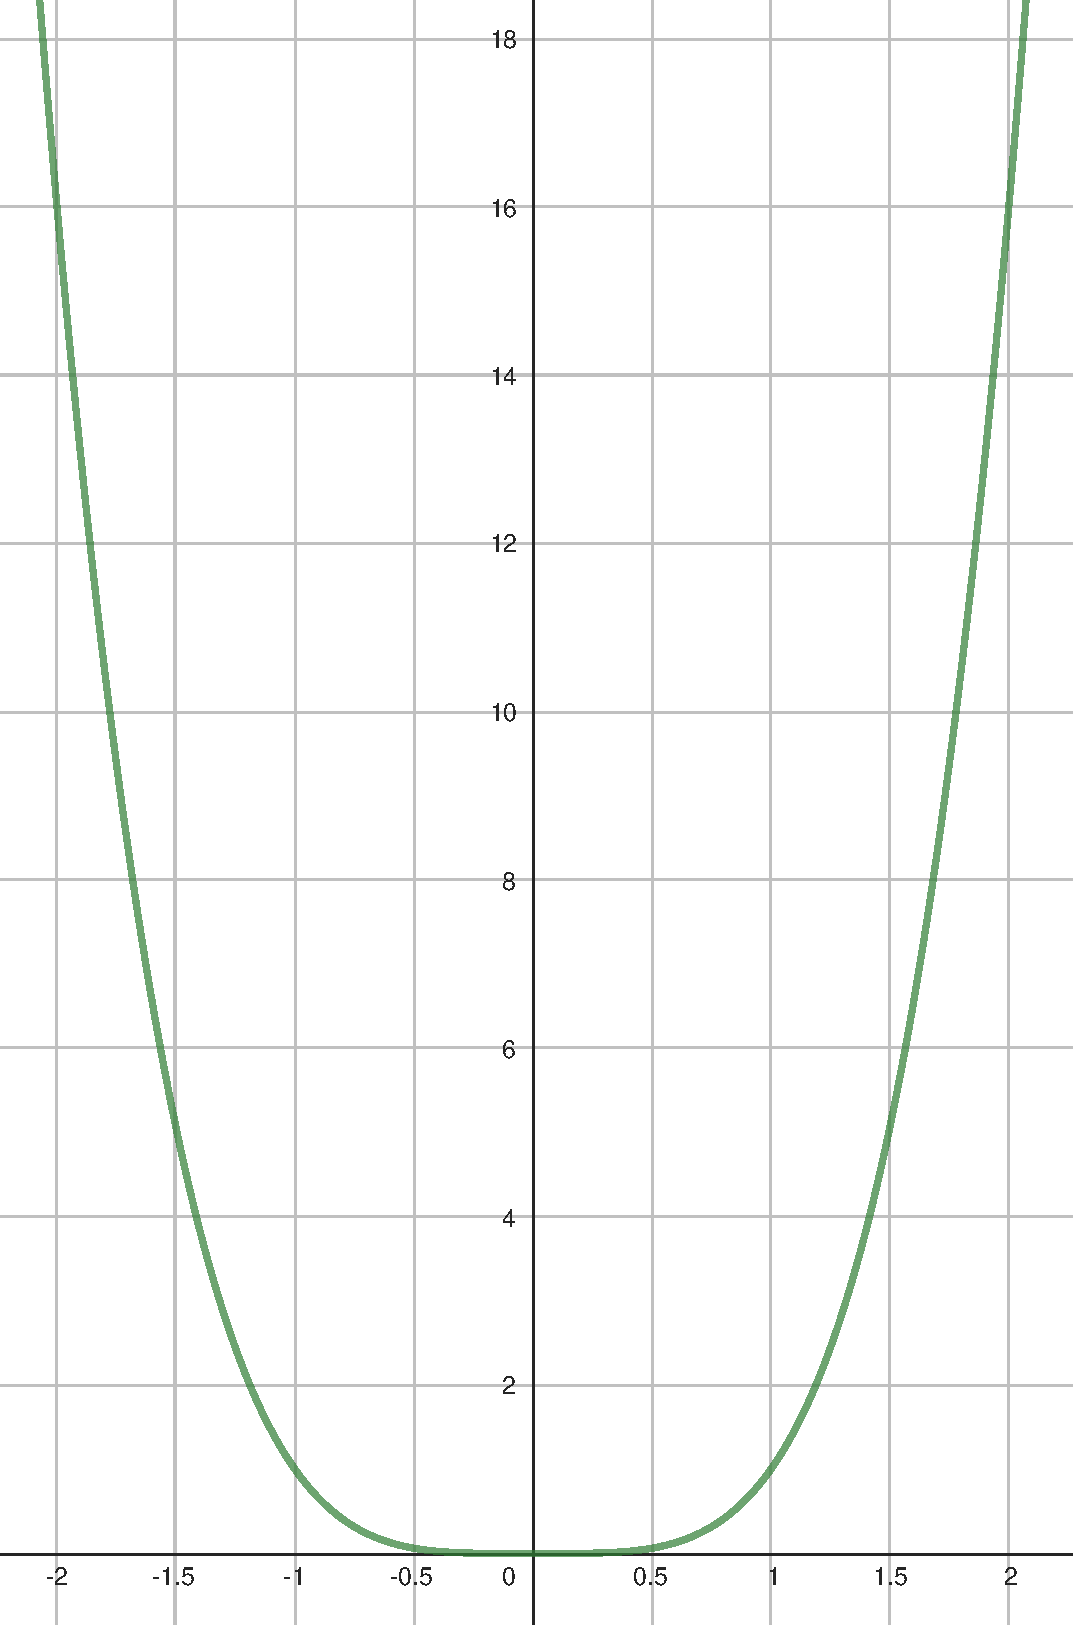
\includegraphics[width=\textwidth]{tex/chapter_2/assets/y=x^4.pdf}
        \caption*{$f(x) = x^4$}
    \end{subfigure}
    \hfill
    \begin{subfigure}{0.35\textwidth}
        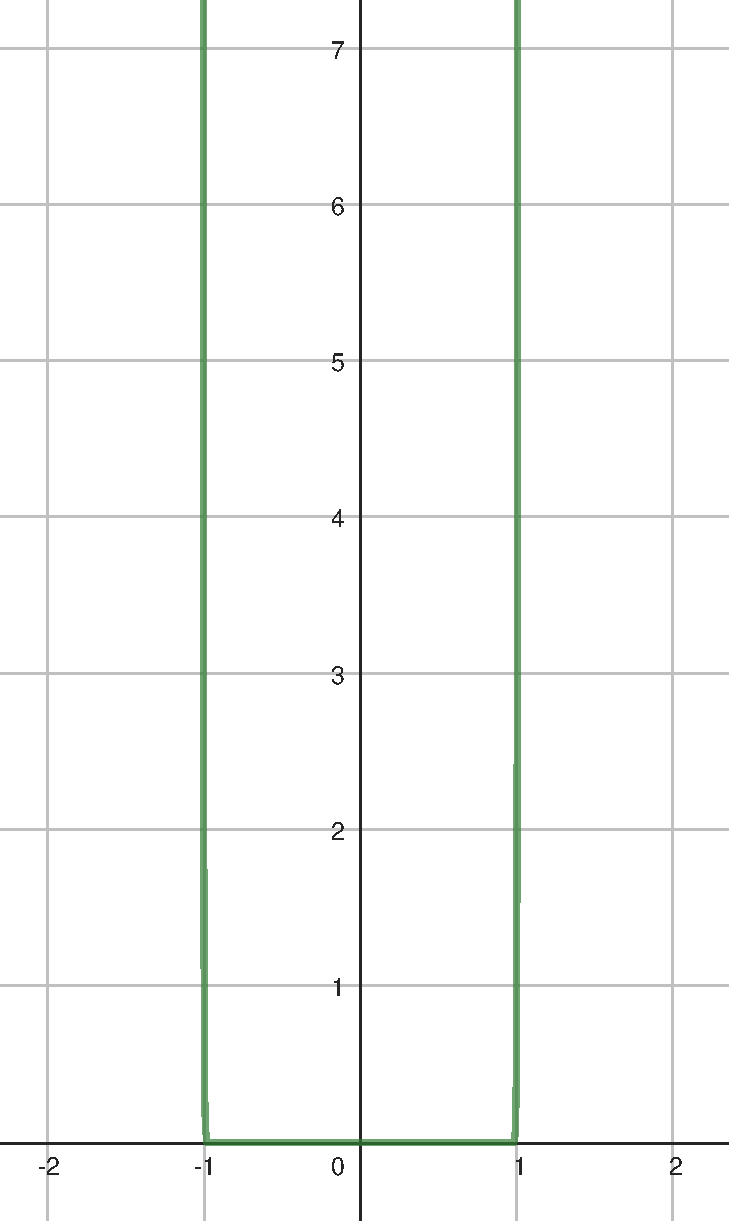
\includegraphics[width=\textwidth]{tex/chapter_2/assets/y=x^300.pdf}
        \caption*{$f(x) = x^{300}$}
    \end{subfigure}
\end{figure}

\subsection{Привет, это Гипербола}

$f(x) = x^m, \; m \in \mathbb{Z} \land m < 0 \land m \notdivisible 2 \iff f(x) = \frac{1}{x^n}, \; n = -m \land n \in \mathbb{N} \land n \notdivisible 2$ \\

\begin{itemize}
    \item $D(f) = \mathbb{R} \backslash \{0\}$
    на ноль делить нельзя
    \item $E(f) = \mathbb{R} \backslash \{0\}$
    уравнение $y = \frac{1}{x^n}$ имеет решения только при $x \neq 0$ 
    \item $f \downarrow (-\infty; 0) \land f \downarrow (0; +\infty)$
    \begin{align*}
        &\forall x_1, x_2 \in \mathbb{R} \backslash \{0\}: x_1 > x_2 \\
        &f(x_1) - f(x_2) = \frac{1}{x_1^n} - \frac{1}{x_2^n} = \frac{x_2^n - x_1^n}{x_1^n x_2^n}\\
    \end{align*}
    Тогда
    \begin{align*}
        &\forall x_1, x_2 \in (0; +\infty) \land x_1 > x_2 \\
        &f(x_1) < f(x_2) \Rightarrow f \downarrow (0; +\infty) \\ \\
        &\forall x_1, x_2 \in (-\infty; 0) \land x_1 > x_2 \\
        &f(x_1) < f(x_2) \Rightarrow f \downarrow (-\infty; 0) \\ \\
    \end{align*}
\end{itemize}

\begin{remark}
    Неверно, что $f \downarrow (-\infty; 0) \cup (0; +\infty)$
\end{remark}

\begin{remark}
    С ростом $n$ (и, соотвеетственно с уменьшением $m$) график будет стремится к двум кочергам в первой и третьей четверти плоскости.
\end{remark}

\begin{figure}[h]
    \centering
    \begin{subfigure}{0.35\textwidth}
        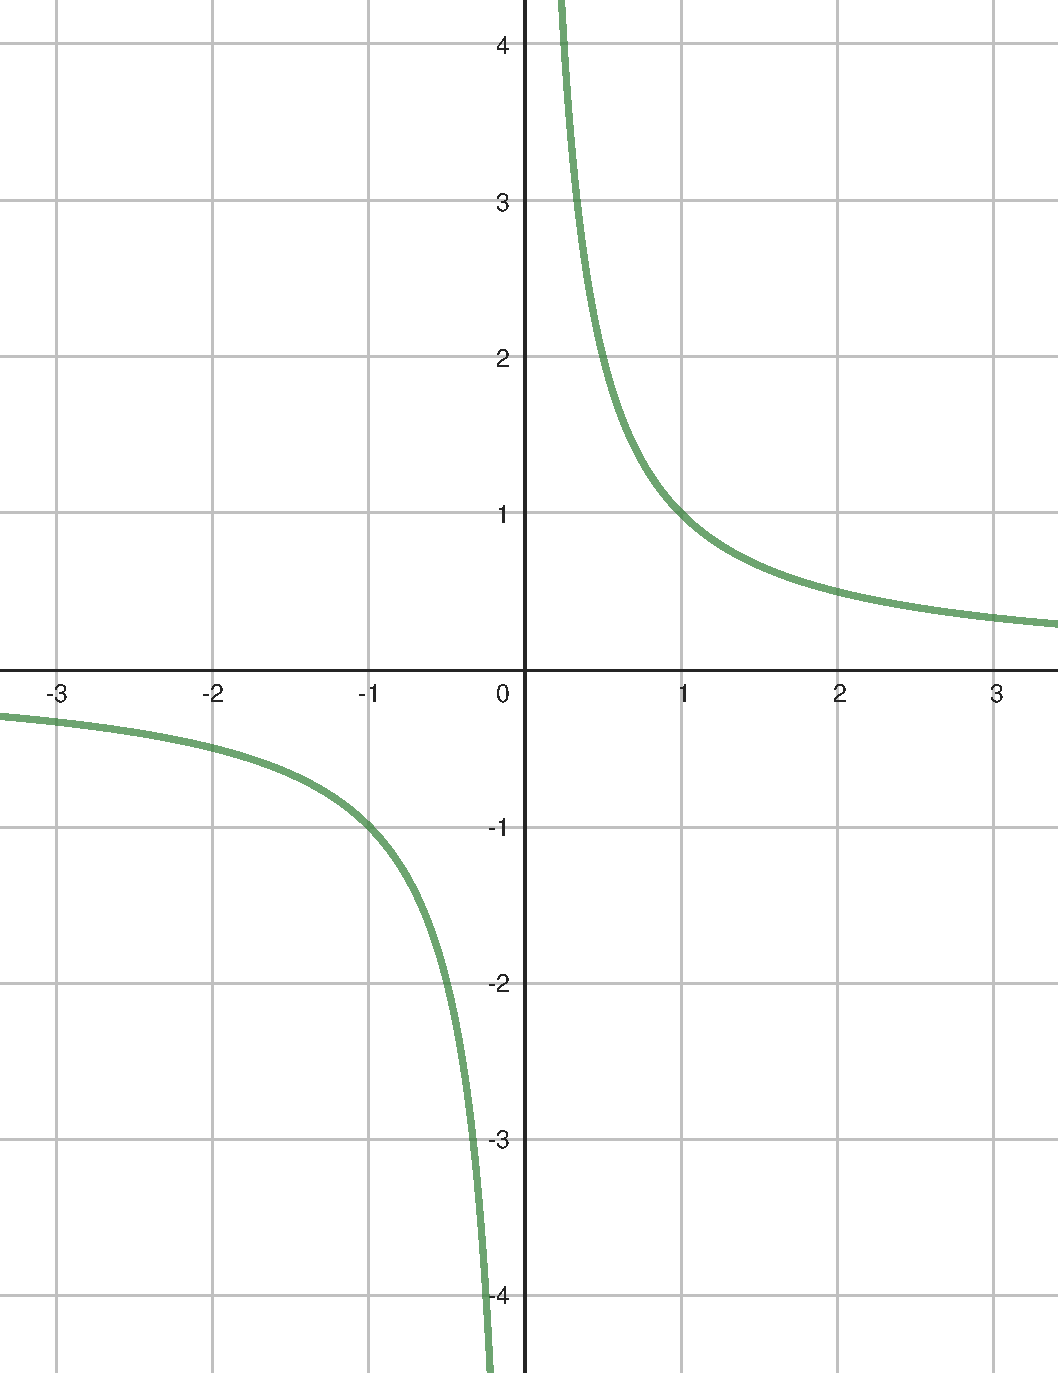
\includegraphics[width=\textwidth]{tex/chapter_2/assets/y=1_div_by_x.pdf}
        \caption*{Гипербола, $f(x) = \frac{1}{x}$}
    \end{subfigure}
    \hfill
    \begin{subfigure}{0.35\textwidth}
        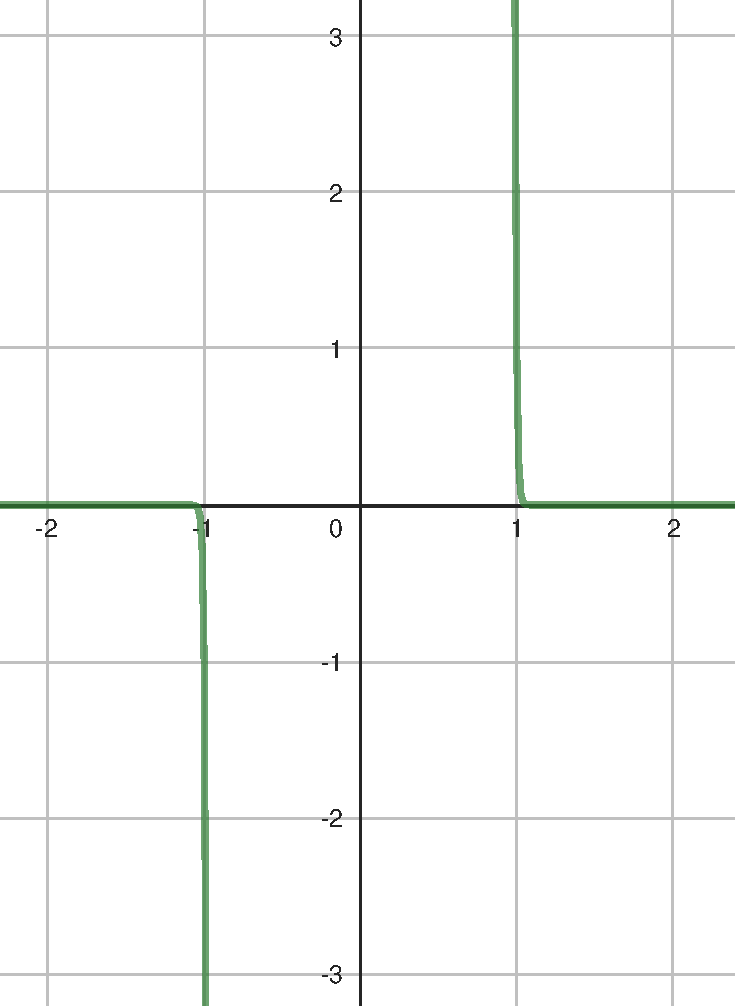
\includegraphics[width=\textwidth]{tex/chapter_2/assets/y=1_div_by_x^99.pdf}
        \caption*{$f(x) = \frac{1}{x^{99}}$, не гипербола}
    \end{subfigure}
\end{figure}

\begin{remark}
    Гиперболой называется график функции $f(x) = \frac{1}{x}$. Другие графики функций вида $f(x) = \frac{1}{x^n}$ не являются гиперболой.
\end{remark}

\subsection{Четная целая отрицательная степень}

$f(x) = x^m, \; m \in \mathbb{Z} \land m < 0 \land m \divisible 2 \iff f(x) = \frac{1}{x^n}, \; n = -m \land n \in \mathbb{N} \land n \divisible 2$ \\

\begin{itemize}
    \item $D(f) = \mathbb{R} \backslash \{0\}$
    \item $E(f) = (0; +\infty)$ уравнение $y = \frac{1}{x^n}$ имеет решения при $y > 0$ тогда $x = \sqrt[n]{\frac{1}{y}}$
    \item $f \uparrow (-\infty; 0) \land f \downarrow (0; +\infty)$
    \begin{align*}
        &\forall x_1, x_2 \in \mathbb{R} \backslash \{0\}: x_1 > x_2 \\
        &f(x_1) - f(x_2) = \frac{1}{x_1^n} - \frac{1}{x_2^n} = \frac{x_2^n - x_1^n}{x_1^n x_2^n}\\
    \end{align*}
    Тогда
    \begin{align*}
        &\forall x_1, x_2 \in (0; +\infty) \land x_1 > x_2 \\
        & f(x_1) - f(x_2) < 0 \iff f(x_1) < f(x_2) \Rightarrow f \downarrow (0; +\infty) \\ \\
        &\forall x_1, x_2 \in (-\infty; 0) \land x_1 > x_2 \\
        & f(x_1) - f(x_2) > 0 \iff f(x_1) > f(x_2) \Rightarrow f \uparrow (-\infty; 0)
    \end{align*}
\end{itemize}

\break

\begin{remark}
    С ростом $n$ (и, соотвеетственно с уменьшением $m$) график будет стремится к двум кочергам в первой и четвертой четверти плоскости.
\end{remark}

\begin{figure}[h]
    \centering
    \begin{subfigure}{0.35\textwidth}
        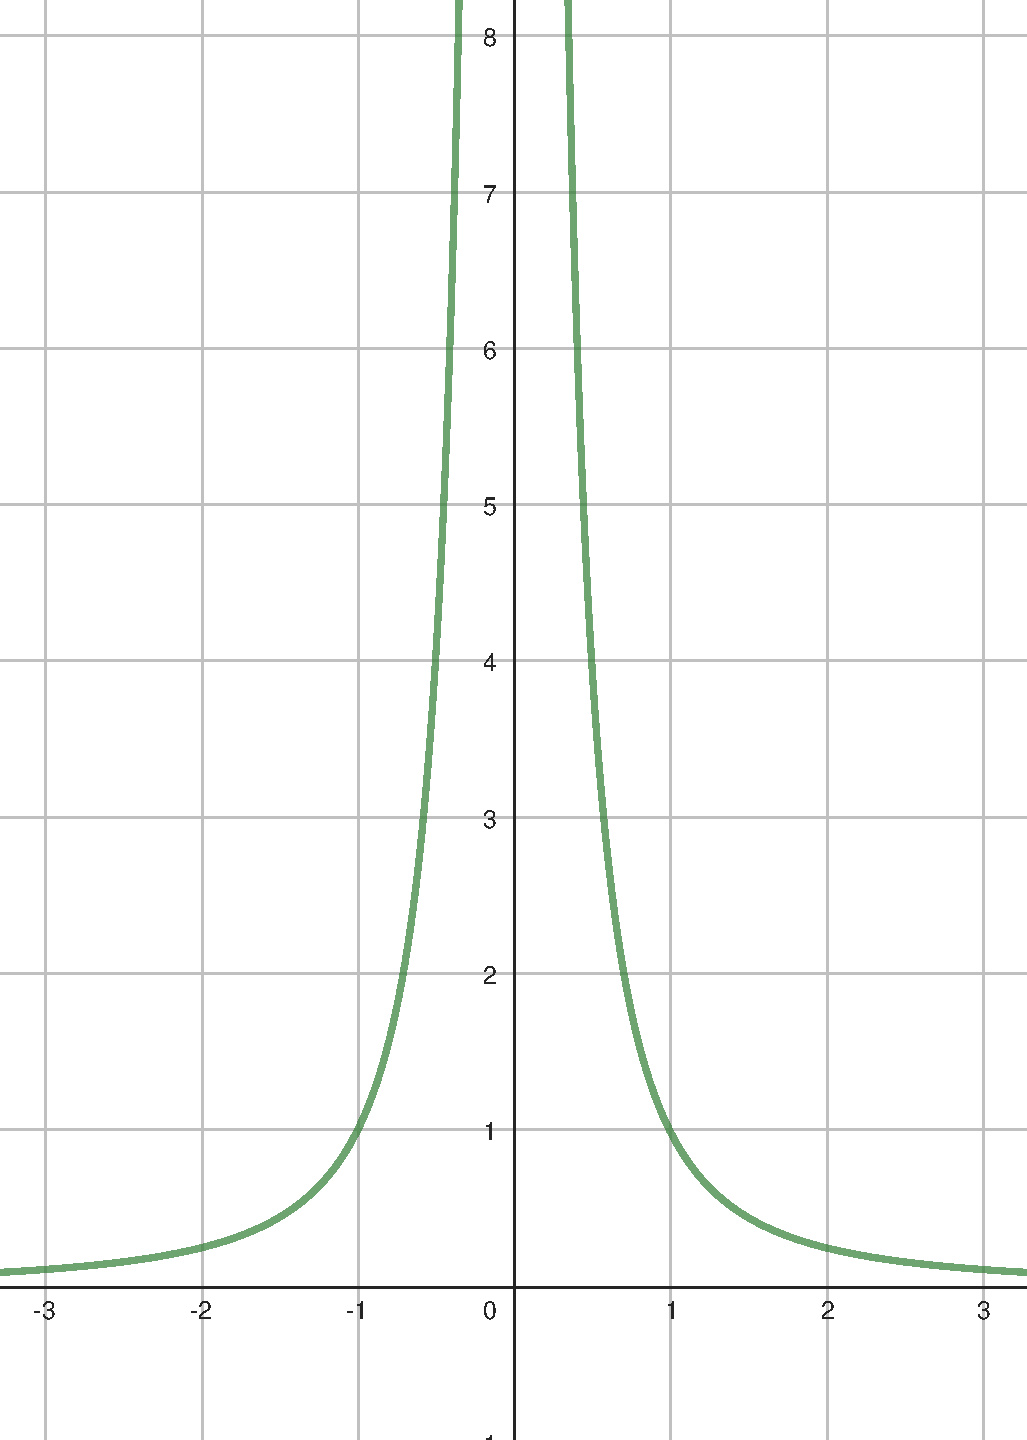
\includegraphics[width=\textwidth]{tex/chapter_2/assets/y=1_div_by_x^2.pdf}
        \caption*{$f(x) = \frac{1}{x^2}$}
    \end{subfigure}
    \hfill
    \begin{subfigure}{0.35\textwidth}
        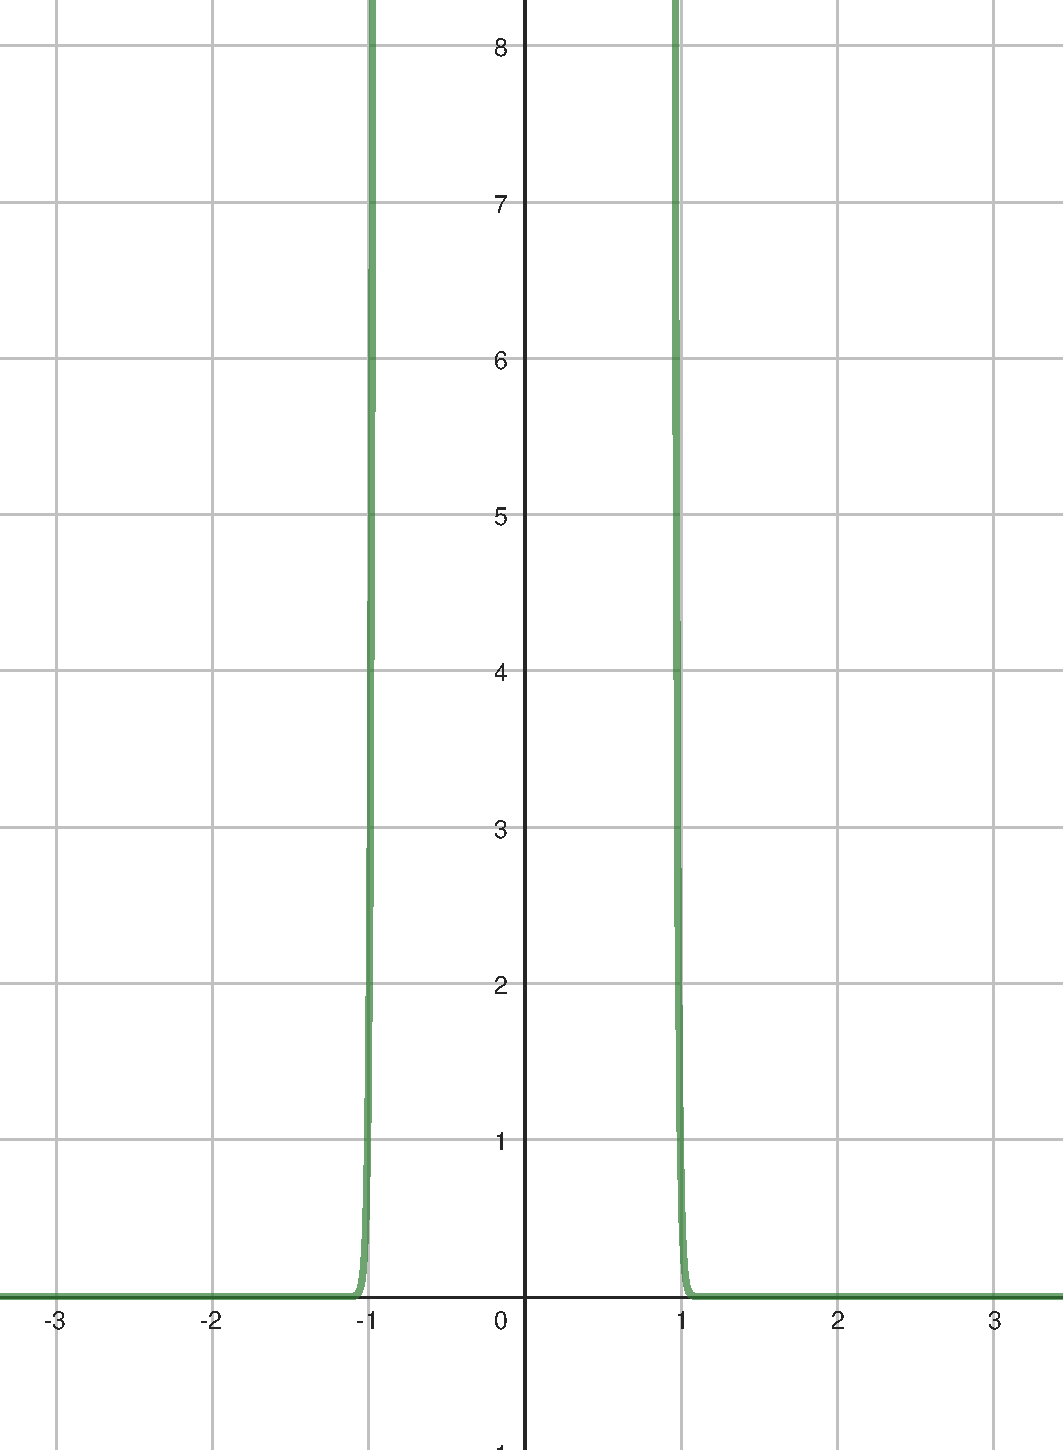
\includegraphics[width=\textwidth]{tex/chapter_2/assets/y=1_div_by_x^64.pdf}
        \caption*{$f(x) = \frac{1}{x^{64}}$}
    \end{subfigure}
\end{figure}

\subsection{Корень нечетной степени}

$f(x) = \sqrt[n]{x}, \; n \in \mathbb{N} \land n \notdivisible 2$

\begin{remark}
    $f(x)^{-1} = x^n$
\end{remark}

\begin{itemize}
    \item $D(f) = \mathbb{R}$
    \item $E(f) = \mathbb{R}$
    \item $f \uparrow \mathbb{R}$
\end{itemize}

\begin{figure}[h]
    \centering
    \begin{subfigure}{0.35\textwidth}
        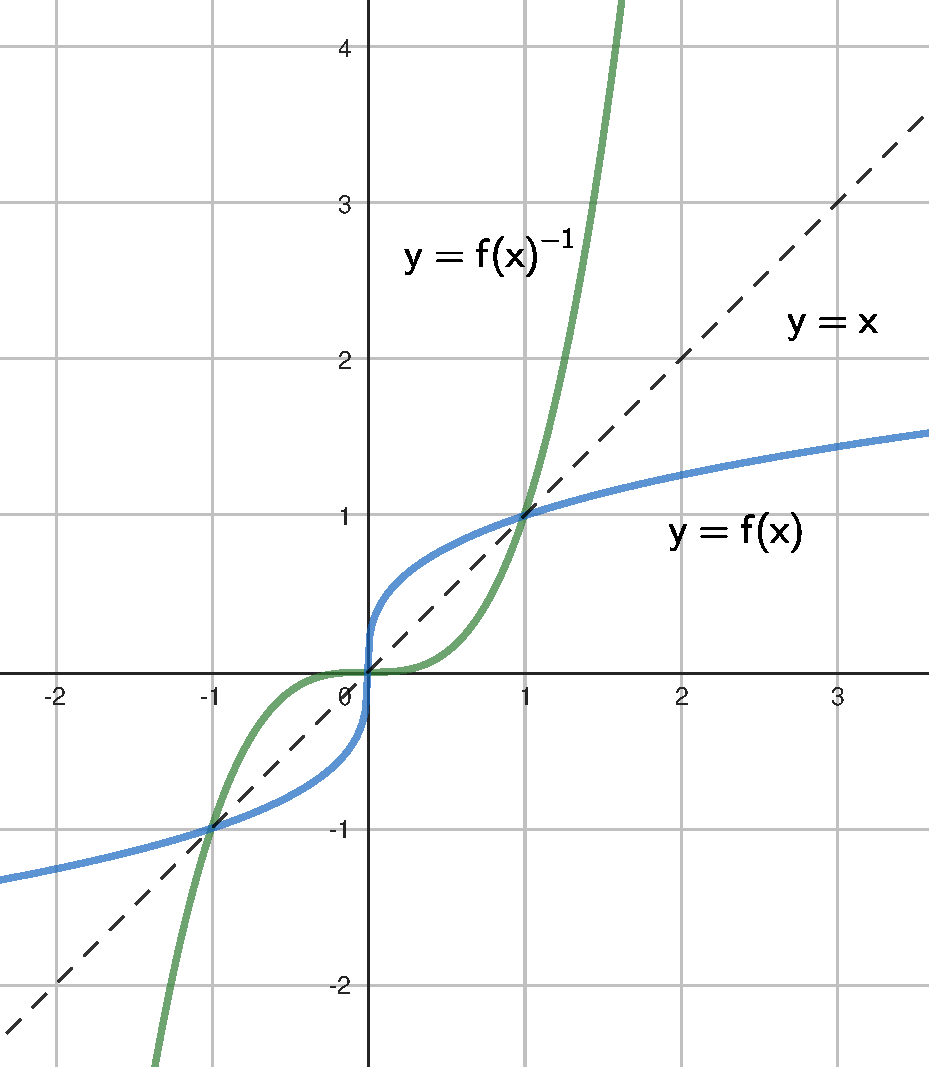
\includegraphics[width=\textwidth]{tex/chapter_2/assets/y=x^(1_div_by_3).pdf}
        \caption*{$f(x) = \sqrt[3]{x}$}
    \end{subfigure}
    \hfill
    \begin{subfigure}{0.5\textwidth}
        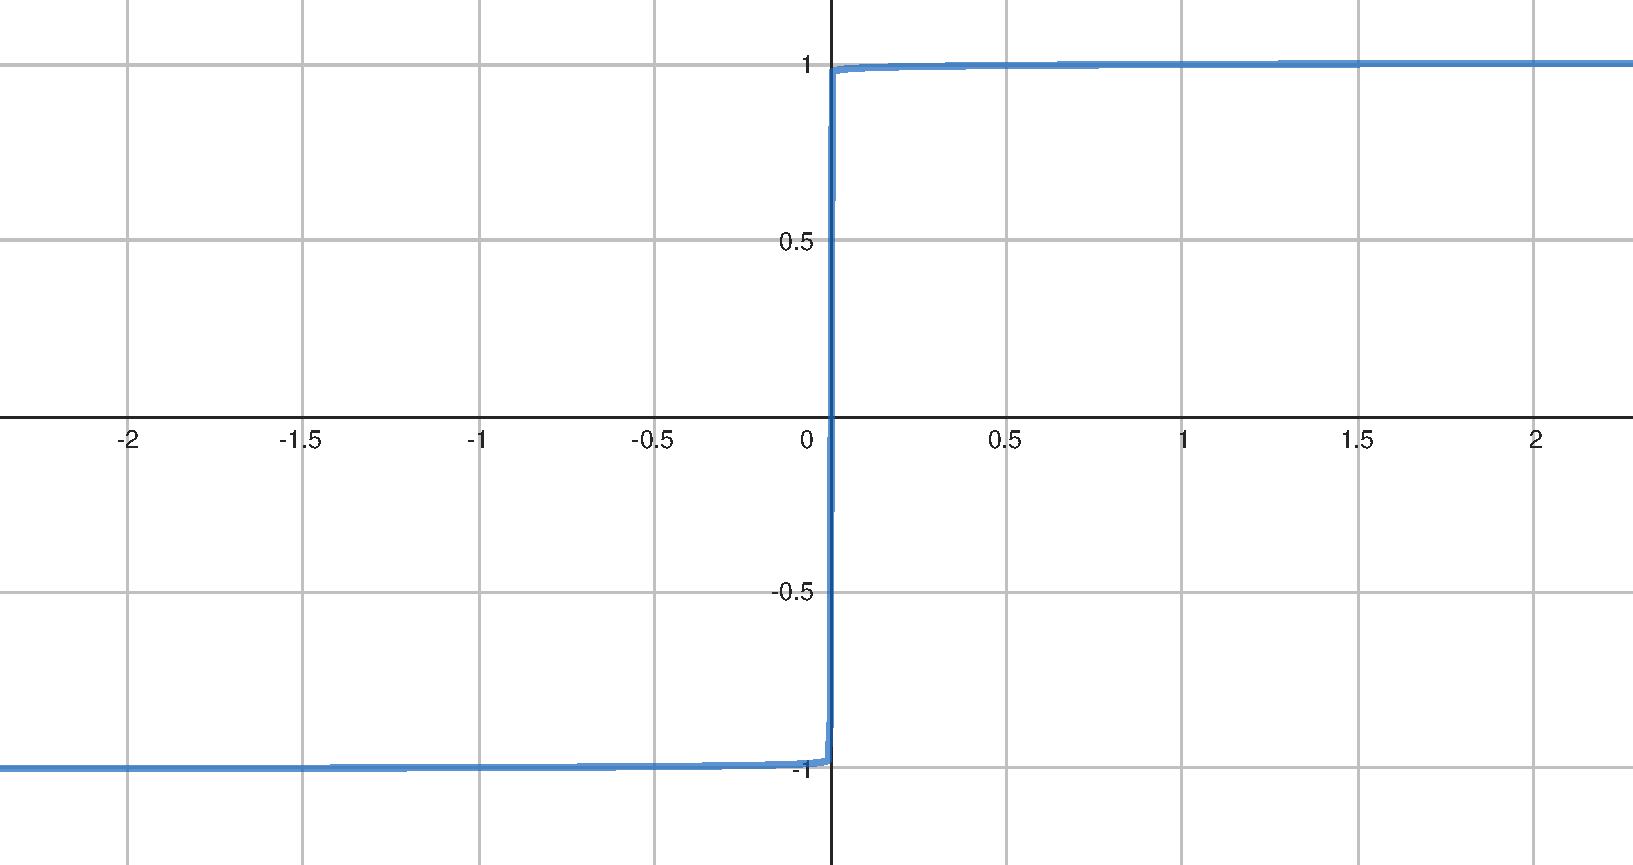
\includegraphics[width=\textwidth]{tex/chapter_2/assets/y=x^(1_div_by_239).pdf}
        \caption*{$f(x) = \sqrt[239]{x}$}
    \end{subfigure}
\end{figure}

\begin{remark}
    С ростом $n$ график будет стремится к кочерге.
\end{remark}

\subsection{Корень четной степени}

$f(x) = \sqrt[n]{x}, \; n \in \mathbb{N} \land n \divisible 2$

\begin{remark}
    $f(x)^{-1} = x^n$ на множестве $[0; +\infty)$
\end{remark}

\begin{itemize}
    \item $D(f) = [0; +\infty)$
    \item $E(f) = [0; +\infty)$
    \item $f \uparrow [0; +\infty)$
\end{itemize}

\begin{remark}
    С ростом $n$ график будет стремится к кочерге.
\end{remark}

\begin{figure}[h]
    \centering
    \begin{subfigure}{0.35\textwidth}
        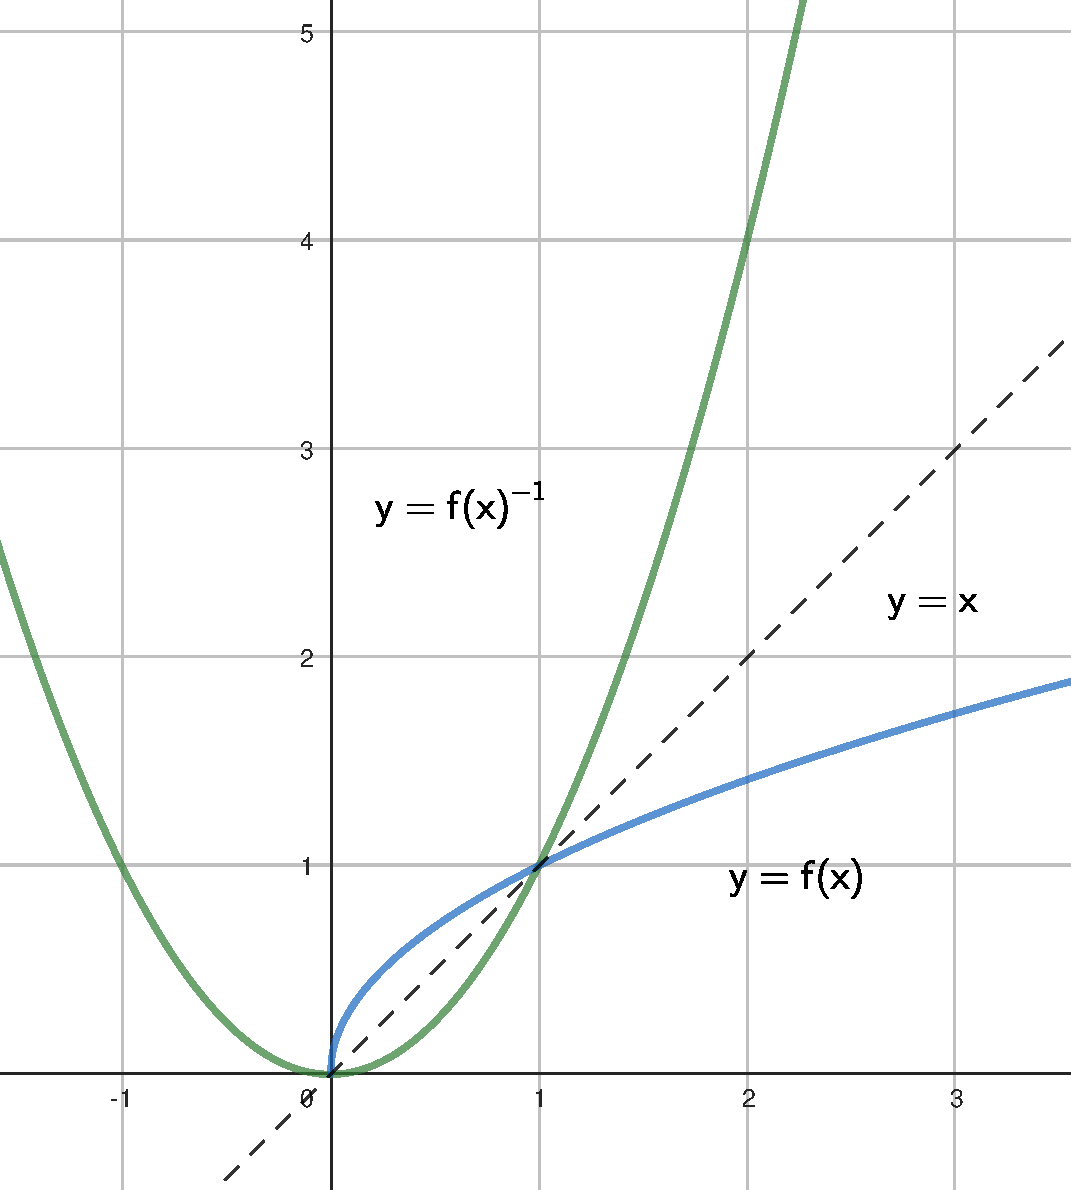
\includegraphics[width=\textwidth]{tex/chapter_2/assets/y=x^(1_div_by_2).pdf}
        \caption*{$f(x) = \sqrt[2]{x}$}
    \end{subfigure}
    \hfill
    \begin{subfigure}{0.5\textwidth}
        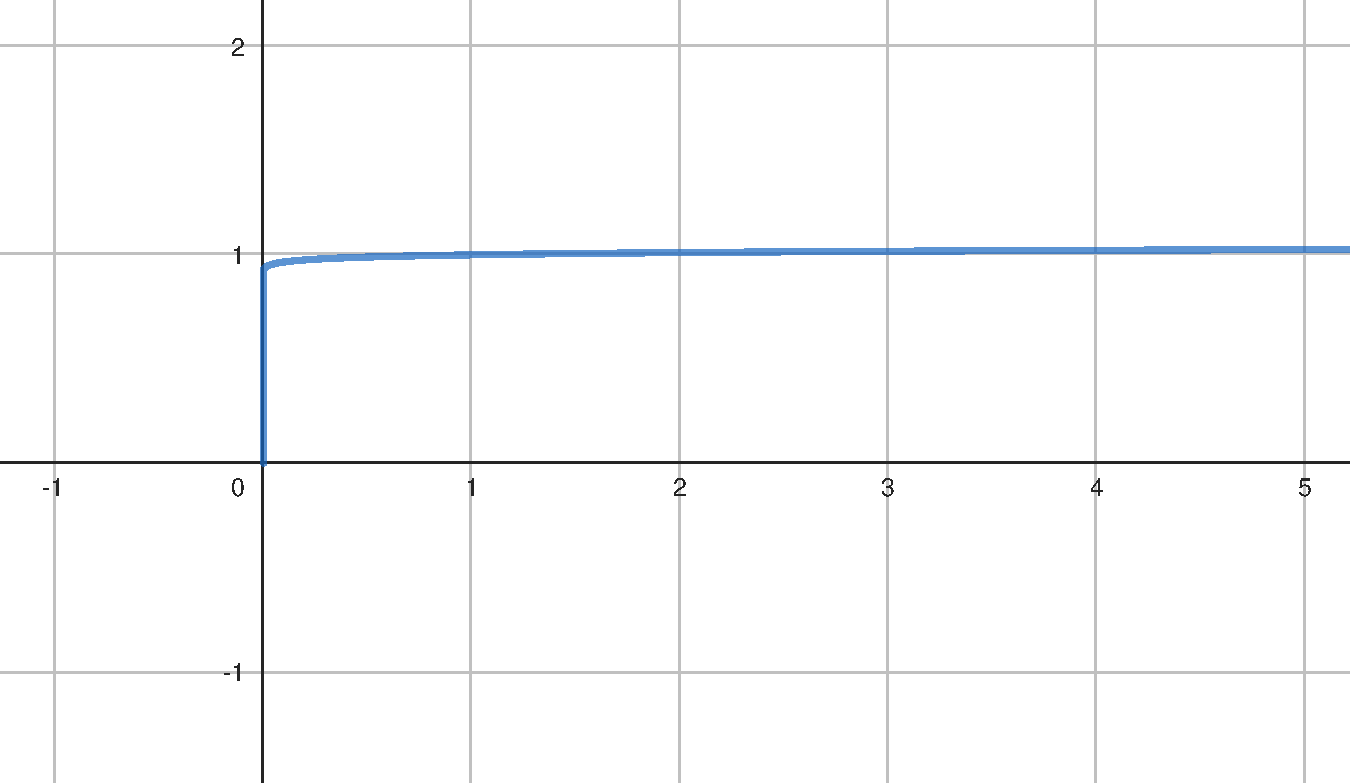
\includegraphics[width=\textwidth]{tex/chapter_2/assets/y=x^(1_div_by_64).pdf}
        \caption*{$f(x) = \sqrt[64]{x}$}
    \end{subfigure}
\end{figure}
	\chapter{Иррациональность}

\section{Иррациональные уравнения}

\begin{align*}
    a = b &\iff f(a) = f(b) \\
    &\Rightarrow - \text{ верно всегда}\\
    &\Leftarrow - \text{ верно, если функция инъективна}
\end{align*}

\begin{definition}[Инъективность]
    Функция называется инъективной на множестве $A$ (инъекция на множестве $A$), если различным значениям аргумента из множества $A$, 
    функция сопостовляет различные значения функции.

    \begin{align*}
        &A \subset D(f) \\
        &\forall x_1, x_2 \in A \;\;\; x_1 \neq x_2 \Rightarrow f(x_1) \neq f(x_2)
    \end{align*}
\end{definition}

\begin{remark}
    На основании теоремы "док-во от обратного":
    \begin{align*}
        &(x_1 \neq x_2 \Rightarrow f(x_1) \neq f(x_2)) \iff (f(x_1) = f(x_2) \Rightarrow x_1 = x_2)
    \end{align*}
\end{remark}

\hfill \newline

\begin{remark}
    График инъективной функции пересекается произвольной горизонтальной прямой не больше одного раза.
\end{remark}

\begin{theorem}[Достаточное условие инъективности]
    Если функция строго монотонна на множестве $A$, то она инъективна на множестве $A$.
\end{theorem}

\begin{proof}
    \begin{align*}
        &\text{Функция строго монотонна, значит } \\
        &\left[\begin{array}{l}
            x < y \iff f(x) < f(y) \\
            x > y \iff f(x) > f(y) 
        \end{array}\right. \Rightarrow
        (x \neq y \iff f(x) \neq f(y))
    \end{align*}
\end{proof}

\begin{remark}
    Обратное неверно!
\end{remark}

\begin{remark}
    Степенная функция с нечетным натуральным показателем -- инъекция на всей вещестенной оси, так как всегда возрастает. 
\end{remark}

\begin{remark}
    Возведение обоих частей уравнения в нечетную натуральную степень всегда будет равносильным преобразованием.
\end{remark}

\begin{remark}
    Степенная функция с четным натуральным показателем не является инъекцией на всей вещестенной оси. 
\end{remark}

\begin{example}
    \begin{align*}
        \text{Если } f(x) = x^4; \; x_1 = 2; \; x_2 = -2, \text{ то } x_1 \neq x_2, \text{ но } f(x_1) = f(x_2) = 16
    \end{align*}
\end{example}

\begin{remark}
    Степенная функция с четным натуральным показателем является инъекцией отдельно на множестве $(-\infty; \; 0]$ и $[0; \; +\infty )$ 
\end{remark}

\begin{remark}
    При возведении обоих частей уравнения в четную натуральную степень могут появится лишние решения.
\end{remark}

\begin{example}
    \begin{align*}
        &\sqrt{x + 2} = x \iff x + 2 = x^2 \iff x^2 - x - 2 = 0 \iff \\
        &\left[\begin{array}{l}
            \uwave{x = -1} \leftarrow \text{лишний корень}\\
            x = 2
        \end{array}\right.
    \end{align*}
\end{example}

\begin{remark}
    Если можем гарантировать, что обе части уравнения имеют одинаковый знак, то возведение их в четную натуральную степень
    будет равносильным преобразованием.
\end{remark}

\begin{example}
    \begin{align*}
        &\sqrt{x + 2} = x \underset{x \ge 0}{\iff} x + 2 = x^2 \iff x^2 - x - 2 = 0 \iff \\
        &\left[\begin{array}{l}
            x = -1 \\
            x = 2
        \end{array}\right. \underset{x \ge 0}{\iff}
        x = 2
    \end{align*}
\end{example}

\begin{example}
    \begin{align*}
        &\sqrt{2x + 7} - \sqrt{x + 3} = 1 \iff \sqrt{2x + 7} = \sqrt{x + 3} + 1 \iff \\
        &2x + 7 = 1 + 2\sqrt{x + 3} + x + 3 \iff 2\sqrt{x + 3} = x + 3 \iff\\
        &4x + 12 = x^2 + 6x + 9 \iff x^2 - 2x - 3 = 0 \iff
        \left[\begin{array}{l}
            x = 1 \\
            x = -3
        \end{array}\right.
    \end{align*}
\end{example}
\section{Иррациональные неравенства}

\begin{align*}
    \begin{array}{c}
        a, b \in A \\
        f \uparrow A
    \end{array}
    \hspace{1.5cm}
    a \le b \iff f(a) \le f(b) \\ \\
    \begin{array}{c}
        a, b \in A \\
        f \downarrow A
    \end{array}
    \hspace{1.5cm}
    a \le b \iff f(a) \ge f(b) \\
\end{align*}

\begin{remark}
    Возведение обоих частей неравенства в нечетную положительную степень всегда является равносильным преобразованием.
\end{remark}

\begin{remark}
    Если обе части неравенства неотрицательны, то их можно возводить в четную натуральную степень, но возможно потребуются ограничения по ОДЗ.
\end{remark}

\begin{example}
    $\sqrt{x - 2} > 3 \iff x - 2 > 9 \iff x > 11$
\end{example}

\begin{example}
    \begin{align*}
        &\sqrt{x - 2} \le 3 \iff
        \left\{\begin{array}{l}
            x - 2 \ge 0 \\
            x - 2  \le 9
        \end{array}\right. \iff
        \left\{\begin{array}{l}
            x \ge 2 \\
            x \le 11
        \end{array}\right. \iff
        x \in [2; 11]
    \end{align*}
\end{example}

\begin{remark}
    Если обе части неравенства неположительные числа, то неравенство можно возвести в четную натуральную степень, 
    но знак неравенства поменяется на противположгный
\end{remark}

\begin{remark}
    Если обе части неравенства имеют разный знак, то их нельзя возводить в четную натуральную степень, но при этом о выполнении неравенства
    можно непосредственно судить.
\end{remark}

\begin{example}
    \begin{align*}
        &\sqrt{x - 2} \le -x \iff
        \left\{\begin{array}{l}
            x \le 0 \\
            x - 2 \le x^2 \\
            x + 2 \ge 0
        \end{array}\right. \iff
        \left\{\begin{array}{l}
            x \in [-2; 0] \\
            (x + 1)(x - 2) \ge 0
        \end{array}\right. \iff
        \left\{\begin{array}{l}
            x \in [-2; 0] \\
            x \in (-\infty; -1] \cup [2; +\infty) \ge 0
        \end{array}\right. \\
        &\text{Ответ: } [-2; -1]
    \end{align*}
\end{example}

\begin{example}
    \begin{align*}
        &\sqrt{x - 2} \ge -x \iff
        \left[
            \begin{array}{l}
                \left\{\begin{array}{l}
                    x > 0 \\
                    x \ge -2
                \end{array}\right. \\
                \left\{\begin{array}{l}
                    x \le 0 \\
                    x + 2 \ge x^2
                \end{array}\right.
            \end{array}
        \right. \iff
        \left[
            \begin{array}{l}
                x \ge -2 \\
                \left\{\begin{array}{l}
                    x \le 0 \\
                    (x + 1)(x - 2) \le 0
                \end{array}\right.
            \end{array}
        \right. \iff
        \left[
            \begin{array}{l}
                x \ge -2 \\
                \left\{\begin{array}{l}
                    x \le 0 \\
                    x \in [-1; 2]
                \end{array}\right.
            \end{array}
        \right. \\
        &\text{Ответ: } [-1; +\infty)
    \end{align*}
\end{example}


\end{document}

